\documentclass{article}
\usepackage[utf8]{inputenc}
\usepackage{amsmath} 
\usepackage{float}
\usepackage{fancyhdr}
\usepackage{lastpage}
\usepackage{lineno}
\usepackage{lmodern}
\usepackage[T1]{fontenc}
\usepackage[utf8]{inputenc}
\usepackage{microtype}
\usepackage{systeme}
\usepackage{amsmath,amssymb,amsthm,mathrsfs,latexsym,tikz,url}
\usepackage{epigraph,graphicx}
%\usepackage{titlesec} %For formatting sections
\usepackage{listings}
\usepackage{listingsutf8}
\usepackage{color}
\usepackage{todonotes}
\presetkeys%
    {todonotes}%
    {inline,backgroundcolor=yellow}{}

\graphicspath{ {./}{./figures/} {images/}}
\DeclareGraphicsExtensions{.png,.pdf}

\definecolor{dkgreen}{rgb}{0,0.6,0}
\definecolor{gray}{rgb}{0.5,0.5,0.5}
\definecolor{mauve}{rgb}{0.58,0,0.82}

\lstset{frame=tb,
  language=Python,
  aboveskip=3mm,
  belowskip=3mm,
  showstringspaces=false,
  columns=flexible,
  basicstyle={\small\ttfamily},
  numbers=none,
  numberstyle=\tiny\color{gray},
  keywordstyle=\color{blue},
  commentstyle=\color{dkgreen},
  stringstyle=\color{mauve},
  breaklines=true,
  breakatwhitespace=true,
  tabsize=4
}


\setlength{\parindent}{0.0cm}
\setlength{\parskip}{0.1cm}


\begin{document}

\title{Lab 3 Machine Learning}
\author{Anton Stråhle \& Jan Alexandersson}
\maketitle

\section*{Assignment 1}

In the function \texttt{mlParams} below we evaluate the $C \times d$ array $\boldsymbol\mu$ and the $C \times d \times d$ array $\boldsymbol\Sigma$ made up of the mean vectors $\boldsymbol\mu_k$ and the covariance matrices $\boldsymbol\Sigma_k$. The expressions for the mean vectors and the covariance matrices are derived through likelihood methods from bivariate Gaussian distributions.

\begin{lstlisting}
def mlParams(X, labels, W=None):
    assert(X.shape[0]==labels.shape[0])
    Npts,Ndims = np.shape(X)
    classes = np.unique(labels)
    Nclasses = np.size(classes)

    if W is None:
        W = np.ones((Npts,1))/float(Npts)

    mu = np.zeros((Nclasses,Ndims))
    sigma = np.zeros((Nclasses,Ndims,Ndims))
    
    for k in range(Nclasses):
        
        ind = np.where(labels == classes[k])[0]
        
        mu[k] = np.sum(X[ind,]*W[ind], axis = 0)/np.sum(W[ind])
        
        sigma[k] = np.diag(np.sum(W[ind]*np.power(X-mu[k],2)[ind],
        axis = 0)/np.sum(W[ind]))   
                          
    return mu, sigma
\end{lstlisting}

We can apply the function \texttt{mlParams} for data consisting of several bivariate Gaussian distributions and then plot the corresponding $95\%$ confidence intervals for the respective distributions.

\begin{figure}
    \centering
    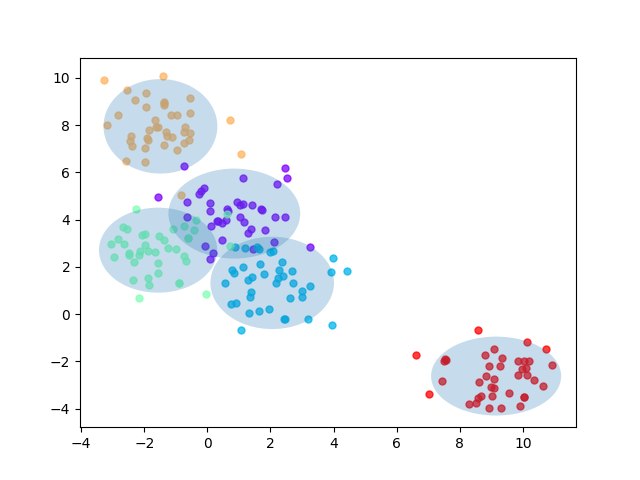
\includegraphics[height=100mm, width=100mm]{Figure_1.png}
    \caption{Gaussian Confidence Intervals}
\end{figure}


\section*{Assignment 2}

In the function \texttt{computePrior} below we calculate the prior probabilities for each of the respective labels. 

\begin{lstlisting}
def computePrior(labels, W=None):
    Npts = labels.shape[0]
    if W is None:
        W = np.ones((Npts,1))/Npts
    else:
        assert(W.shape[0] == Npts)
    classes = np.unique(labels)
    Nclasses = np.size(classes)

    prior = np.zeros((Nclasses,1))
    
    for k in range(Nclasses):
        
        ind = np.where(labels == classes[k])[0]
        
        prior[k] = np.sum(W[ind])/np.sum(W)

    return prior
\end{lstlisting}

Using the previous function \texttt{mlParams} to compute the arrays $\boldsymbol\mu$ and $\boldsymbol\Sigma$ we can use \texttt{computePrior} to evaluate the posterior probabilities in the function \texttt{classifyBayes} which uses a naive Bayes classifier to classify a set of points \texttt{X}.

\begin{lstlisting}
def classifyBayes(X, prior, mu, sigma):

    Npts = X.shape[0]
    Nclasses,Ndims = np.shape(mu)
    logProb = np.zeros((Nclasses, Npts))
    
    for k in range(Nclasses):
        
        diff = X-mu[k]
        
        logSigma = np.log(np.linalg.det(sigma[k]))/2
        
        logPrior = np.log(prior[k])
        
        for j in range(Npts):
            
            logProb[k][j] = -logSigma - np.inner(diff[j]/np.diag(sigma[k]), diff[j])/2 + logPrior

    h = np.argmax(logProb,axis=0)
    return h
\end{lstlisting}

\section*{Assignment 3}

We can use the aforementioned function \texttt{classifyBayes} to test how well it performs on separate data sets. The data sets that we have available are one containing data of different types of irises and one contains data for different vowels. 

We can plot the classification boundaries for the respective data sets as follows.

\begin{figure}
    \centering
    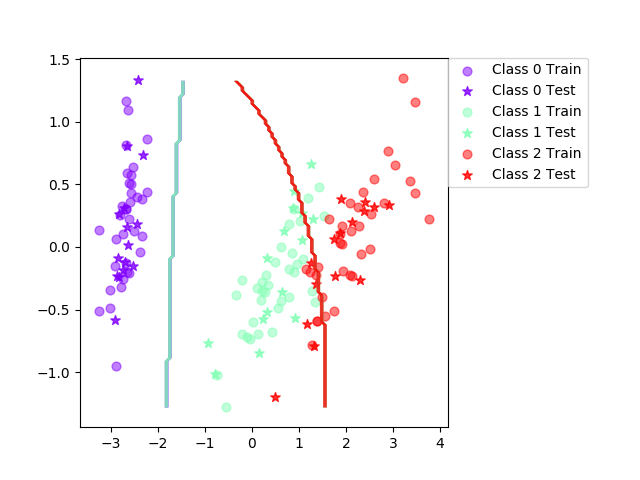
\includegraphics[scale = 0.90]{BayesIris.png}
    \caption{Bayes Classifier: Iris}
\end{figure}

When using the naive Bayes classifier for the iris data set we get that the trained classifier has a mean classification accuracy of 89 with a standard deviation of 4.16.

\begin{figure}
    \centering
    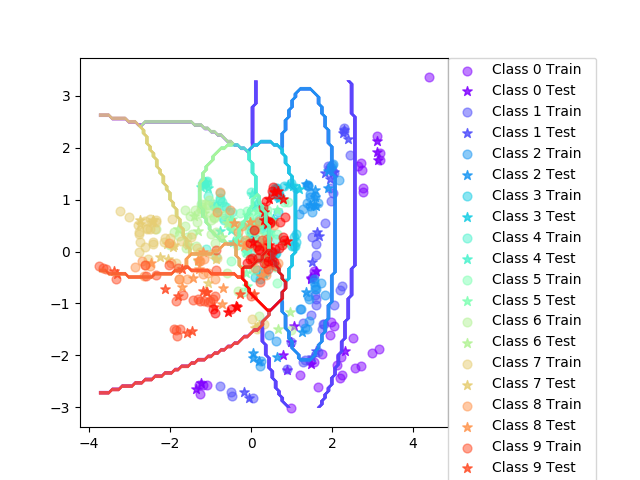
\includegraphics[scale = 0.90]{BayesVowel.png}
    \caption{Bayes Classifier: Vowel}
\end{figure}

When using the naive Bayes classifier for the vowel data set we get that the trained classifier has a mean classification accuracy of 64.7 with a standard deviation of 4.03. It is not unexpected that the classifier has a higher accuracy for the iris data set compared to the vowel data set since the number of valid targets are much lower for the iris data set, specifically 3 compared to 11.

Feature independence, which is assumed in the naive Bayes classifier, is independence between the features conditioned on the class. In Figure 2 we observe that the features represented on the $x$ and $y$-axis could be said to be independent conditioned on Class 0. If we however observe Classes 1 and 2 instead we note that there is a clear linear dependency between the features, meaning that the assumption is not satisfied. 

In the iris data set presented in Figure 2 we note that Classes 1 and 2 seem to overlap slightly. One way to deal with the data, making it more separable, could be to transform it into higher dimension. It could also be possible to boost the algorithm, as will be done later on, in order to improve the boundary. 

\section*{Assignment 4 \& 5}

The rewritten versions of \texttt{mlParams} and \texttt{computePrior} were presented in Assignment 1.

We use these rewritten functions in order to implement the Adaboost algorithm as can be seen below.

The function \texttt{trainBoost} trains the booster.

\begin{lstlisting}
def trainBoost(base_classifier, X, labels, T=10):
    # these will come in handy later on
    Npts,Ndims = np.shape(X)
    
    classes = np.unique(labels)
    
    classifiers = [] # append new classifiers to this list
    alphas = [] # append the vote weight of the classifiers to this list

    # The weights for the first iteration
    wCur = np.ones((Npts,1))/float(Npts)

    for i_iter in range(0, T):
        # a new classifier can be trained like this, given the current weights
        classifiers.append(base_classifier.trainClassifier(X, labels, wCur))

        # do classification for each point
        vote = classifiers[-1].classify(X)
        
        eps = 0.0
        
        for k in classes:
            
            ind = np.where(vote == k)[0]
            
            eps += np.sum(np.transpose(wCur[ind])* (1-(k == labels[ind]))) 
        
        alpha = (np.log(1-eps) - np.log(eps))/2
        
        alphas.append(alpha)
        
        wOld = wCur
        
        for i in range(len(wOld)):
            
            wCur[i] = wOld[i]*np.exp(alpha * np.power(-1,(vote[i] == labels[i])))
        
        wCur = wCur/np.sum(wCur)
        
    return classifiers, alphas
\end{lstlisting}

Whilst the function \texttt{classifyBoost} classifies using the trained booster.

\begin{lstlisting}
def classifyBoost(X, classifiers, alphas, Nclasses):
    Npts = X.shape[0]
    Ncomps = len(classifiers)

    # if we only have one classifier, we may just classify directly
    if Ncomps == 1:
        return classifiers[0].classify(X)
    else:
        votes = np.zeros((Npts,Nclasses))
        
        for j in range(Ncomps):
            
            vote = classifiers[j].classify(X)
            
            for i in range(Npts):
                
                votes[i, vote[i]] += alphas[j]
            
        return np.argmax(votes,axis=1)
\end{lstlisting}

When using a boosted naive Bayes classifiers we get the following boundary.
        
\begin{figure}
    \centering
    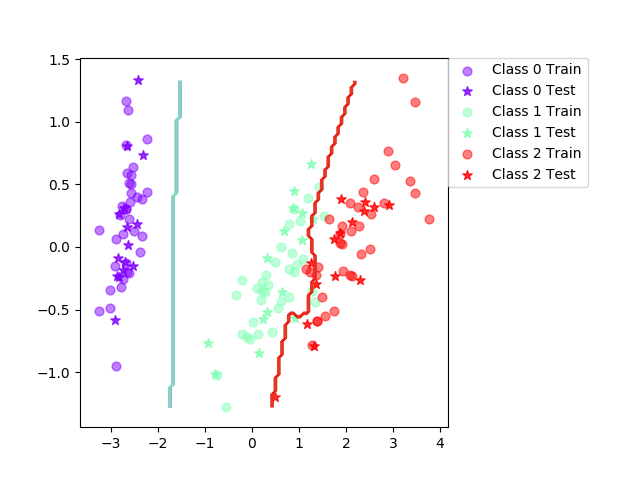
\includegraphics[scale = 0.90]{BoostedBayesIrirs.png}
    \caption{Adaboosted Bayes Classifier: Iris}
\end{figure}

We note that the decision boundary is a lot more complex compared to the non-boosted boundary presented in Figure 2. We also get a slight increase in the mean classification accuracy 94.1 and with standard deviation 6.72 which is an increase from the non-boosted version. Given that our data lacks extreme outliers this is to be expected since every iteration of the Adaboost algorithm aims to improve the classifier by weighting the missclassified data points to subtly be able to incorporate the into the model. The lack of outliers, which Adaboosting has troubles with due to increasing the weight of the always missclassified outliers the model boosting is in some sense expected to improve the accuracy, which it does.

As long as our basic model is better than randomly guessing the label and the data set is has some kind of structure, boosting will be able to partially make up for the lack of complexity in the initial model by tweaking the weights and as such achieve better accuracy. The level of improvement obviously depends on the strength of the initial classifier and the data set in question. It should be noted that boosting "too much" leads to overfitting the data and as such a very weak classifier that requires a lot of boosting might not be able to achieve the same results as another strong classifier due to overfitting.


\section*{Assignment 6}

When implementing the non-boosted decision tree classifier on the iris data set we end up with the following results:

\texttt{Final mean classification accuracy  92.4 with standard deviation 3.71}

When Adaboosting the same classifier we get a slight improvement:

\texttt{Final mean classification accuracy  94.6 with standard deviation 3.65}

We see that the decision tree classifies the iris data quite well even without boosting. When boosting the classifier we only see a slight improvement which would imply that the decision tree could be seen as a strong learner in the case of the iris data.

For the data set with vowels we have got the following results for the non-boosted decision tree:

\texttt{Final mean classification accuracy  64.1 with standard deviation 4}

When Adaboosting the same classifier we get a significant improvement:

\texttt{Final mean classification accuracy  86.6 with standard deviation 3}

Since the initial classifier had a fairly low accuracy it could be classified as a weak learner which given the data set, which seem to lack any extreme outliers as can be seen in Figure 2, leads to a vast improvement when boosting, as can be seen from the results above.

\begin{figure}
    \centering
    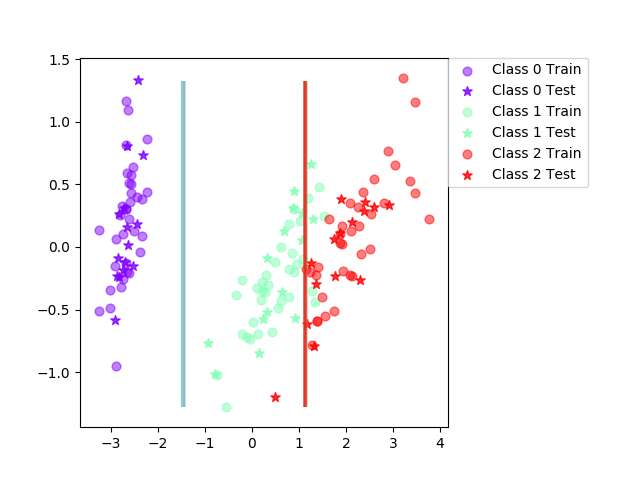
\includegraphics[scale = 0.90]{Dectree.png}
    \caption{Decision Tree Classifier: Iris}
\end{figure}

\begin{figure}
    \centering
    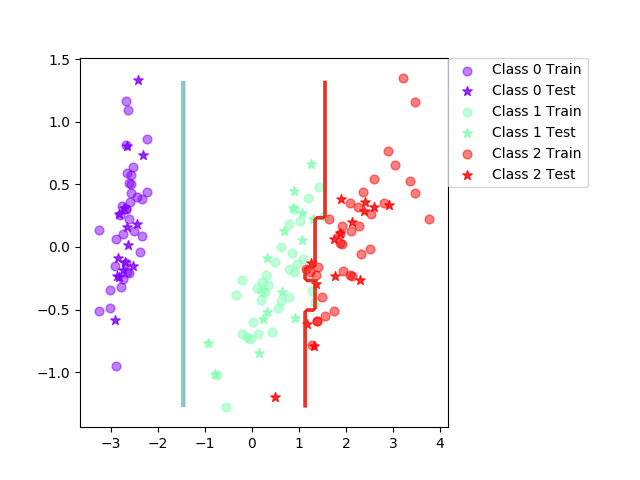
\includegraphics[scale = 0.90]{BoostedDectree.png}
    \caption{Adaboosted Decision Tree Classifier: Iris}
\end{figure}

The non-boosted decision tree classifier seems to only split on the feature presented on the x-axis whilst the Adaboosted tree uses the features on both axes in order to incorporate the initially missclassified data points on between the cluster of class 1 and that of class 2. In this case the boosting of the weak decision tree classifier seems to be able to make up for the choice of a weak classifier in itself.

\section*{Assignment 7}

\begin{itemize}

\item In the case of outliers we should avoid boosting in general since the model will overfit in order to attempt to include the outliers. The choice between naive Bayes or a decision tree depends on the data. E.g. dependent features makes Bayes bad.

\item In the case of a partially irrelevant feature space a decision tree should be chosen as the irrelevant features will in a sense be pruned away. The choice of boosting should depend on how well the decision tree classifies initially.

\item This very much depends on the data. They both have their respective strengths and weaknesses. Decision trees does for example need quite large amounts of data whilst Naive Bayes assumed independent features etc. The decision to boost also depends on data as discussed in the previous points.

\item Decision trees work well with mixed data as they simply split on a threshold. In our case of Gaussian naive Bayes categorical data would not work since the Gaussian distribution is continuous. Since the naive Bayes classifier always assumes an underlying distribution data needs to be on the same form since there exists no distribution that is both contiguous and discrete.

\item In terms of scalability a decision tree works well for large $N$ as previously mentioned. A large number of features $D$ makes the assumption of independent features very unlikely for the naive Bayes classifier whilst a decision tree might work better. Larger $N$ increases the probability of outliers which might lead to overfitting when boosting.

\end{itemize}

\newpage

\section*{Assignment 8: Olivetti Faces}

\begin{figure}
    \centering
    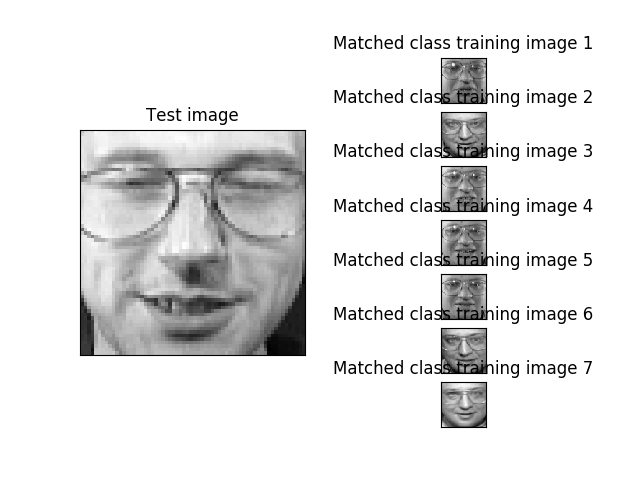
\includegraphics[scale = 0.90]{Olivetti.png}
    \caption{Adaboosted Decision Tree Classifier: Olivetti Spaghetti}
\end{figure}








\end{document}
